\documentclass[twoside]{book}

% Packages required by doxygen
\usepackage{fixltx2e}
\usepackage{calc}
\usepackage{doxygen}
\usepackage{graphicx}
\usepackage[utf8]{inputenc}
\usepackage{makeidx}
\usepackage{multicol}
\usepackage{multirow}
\PassOptionsToPackage{warn}{textcomp}
\usepackage{textcomp}
\usepackage[nointegrals]{wasysym}
\usepackage[table]{xcolor}

% Font selection
\usepackage[T1]{fontenc}
\usepackage{mathptmx}
\usepackage[scaled=.90]{helvet}
\usepackage{courier}
\usepackage{amssymb}
\usepackage{sectsty}
\renewcommand{\familydefault}{\sfdefault}
\allsectionsfont{%
  \fontseries{bc}\selectfont%
  \color{darkgray}%
}
\renewcommand{\DoxyLabelFont}{%
  \fontseries{bc}\selectfont%
  \color{darkgray}%
}
\newcommand{\+}{\discretionary{\mbox{\scriptsize$\hookleftarrow$}}{}{}}

% Page & text layout
\usepackage{geometry}
\geometry{%
  a4paper,%
  top=2.5cm,%
  bottom=2.5cm,%
  left=2.5cm,%
  right=2.5cm%
}
\tolerance=750
\hfuzz=15pt
\hbadness=750
\setlength{\emergencystretch}{15pt}
\setlength{\parindent}{0cm}
\setlength{\parskip}{0.2cm}
\makeatletter
\renewcommand{\paragraph}{%
  \@startsection{paragraph}{4}{0ex}{-1.0ex}{1.0ex}{%
    \normalfont\normalsize\bfseries\SS@parafont%
  }%
}
\renewcommand{\subparagraph}{%
  \@startsection{subparagraph}{5}{0ex}{-1.0ex}{1.0ex}{%
    \normalfont\normalsize\bfseries\SS@subparafont%
  }%
}
\makeatother

% Headers & footers
\usepackage{fancyhdr}
\pagestyle{fancyplain}
\fancyhead[LE]{\fancyplain{}{\bfseries\thepage}}
\fancyhead[CE]{\fancyplain{}{}}
\fancyhead[RE]{\fancyplain{}{\bfseries\leftmark}}
\fancyhead[LO]{\fancyplain{}{\bfseries\rightmark}}
\fancyhead[CO]{\fancyplain{}{}}
\fancyhead[RO]{\fancyplain{}{\bfseries\thepage}}
\fancyfoot[LE]{\fancyplain{}{}}
\fancyfoot[CE]{\fancyplain{}{}}
\fancyfoot[RE]{\fancyplain{}{\bfseries\scriptsize Generated on Sun Dec 7 2014 14\+:18\+:14 for Key\+Player by Doxygen }}
\fancyfoot[LO]{\fancyplain{}{\bfseries\scriptsize Generated on Sun Dec 7 2014 14\+:18\+:14 for Key\+Player by Doxygen }}
\fancyfoot[CO]{\fancyplain{}{}}
\fancyfoot[RO]{\fancyplain{}{}}
\renewcommand{\footrulewidth}{0.4pt}
\renewcommand{\chaptermark}[1]{%
  \markboth{#1}{}%
}
\renewcommand{\sectionmark}[1]{%
  \markright{\thesection\ #1}%
}

% Indices & bibliography
\usepackage{natbib}
\usepackage[titles]{tocloft}
\setcounter{tocdepth}{3}
\setcounter{secnumdepth}{5}
\makeindex

% Hyperlinks (required, but should be loaded last)
\usepackage{ifpdf}
\ifpdf
  \usepackage[pdftex,pagebackref=true]{hyperref}
\else
  \usepackage[ps2pdf,pagebackref=true]{hyperref}
\fi
\hypersetup{%
  colorlinks=true,%
  linkcolor=blue,%
  citecolor=blue,%
  unicode%
}

% Custom commands
\newcommand{\clearemptydoublepage}{%
  \newpage{\pagestyle{empty}\cleardoublepage}%
}


%===== C O N T E N T S =====

\begin{document}

% Titlepage & ToC
\hypersetup{pageanchor=false,
             bookmarks=true,
             bookmarksnumbered=true,
             pdfencoding=unicode
            }
\pagenumbering{roman}
\begin{titlepage}
\vspace*{7cm}
\begin{center}%
{\Large Key\+Player }\\
\vspace*{1cm}
{\large Generated by Doxygen 1.8.8}\\
\vspace*{0.5cm}
{\small Sun Dec 7 2014 14:18:14}\\
\end{center}
\end{titlepage}
\clearemptydoublepage
\tableofcontents
\clearemptydoublepage
\pagenumbering{arabic}
\hypersetup{pageanchor=true}

%--- Begin generated contents ---
\chapter{Hierarchical Index}
\section{Class Hierarchy}
This inheritance list is sorted roughly, but not completely, alphabetically\+:\begin{DoxyCompactList}
\item P\+Applet\begin{DoxyCompactList}
\item \contentsline{section}{keyplayer\+\_\+gui}{\pageref{classkeyplayer__gui}}{}
\end{DoxyCompactList}
\end{DoxyCompactList}

\chapter{Class Index}
\section{Class List}
Here are the classes, structs, unions and interfaces with brief descriptions\+:\begin{DoxyCompactList}
\item\contentsline{section}{\hyperlink{classkeyplayer__gui}{keyplayer\+\_\+gui} }{\pageref{classkeyplayer__gui}}{}
\end{DoxyCompactList}

\chapter{Class Documentation}
\hypertarget{classkeyplayer}{\section{keyplayer Class Reference}
\label{classkeyplayer}\index{keyplayer@{keyplayer}}
}
Inheritance diagram for keyplayer\+:\begin{figure}[H]
\begin{center}
\leavevmode
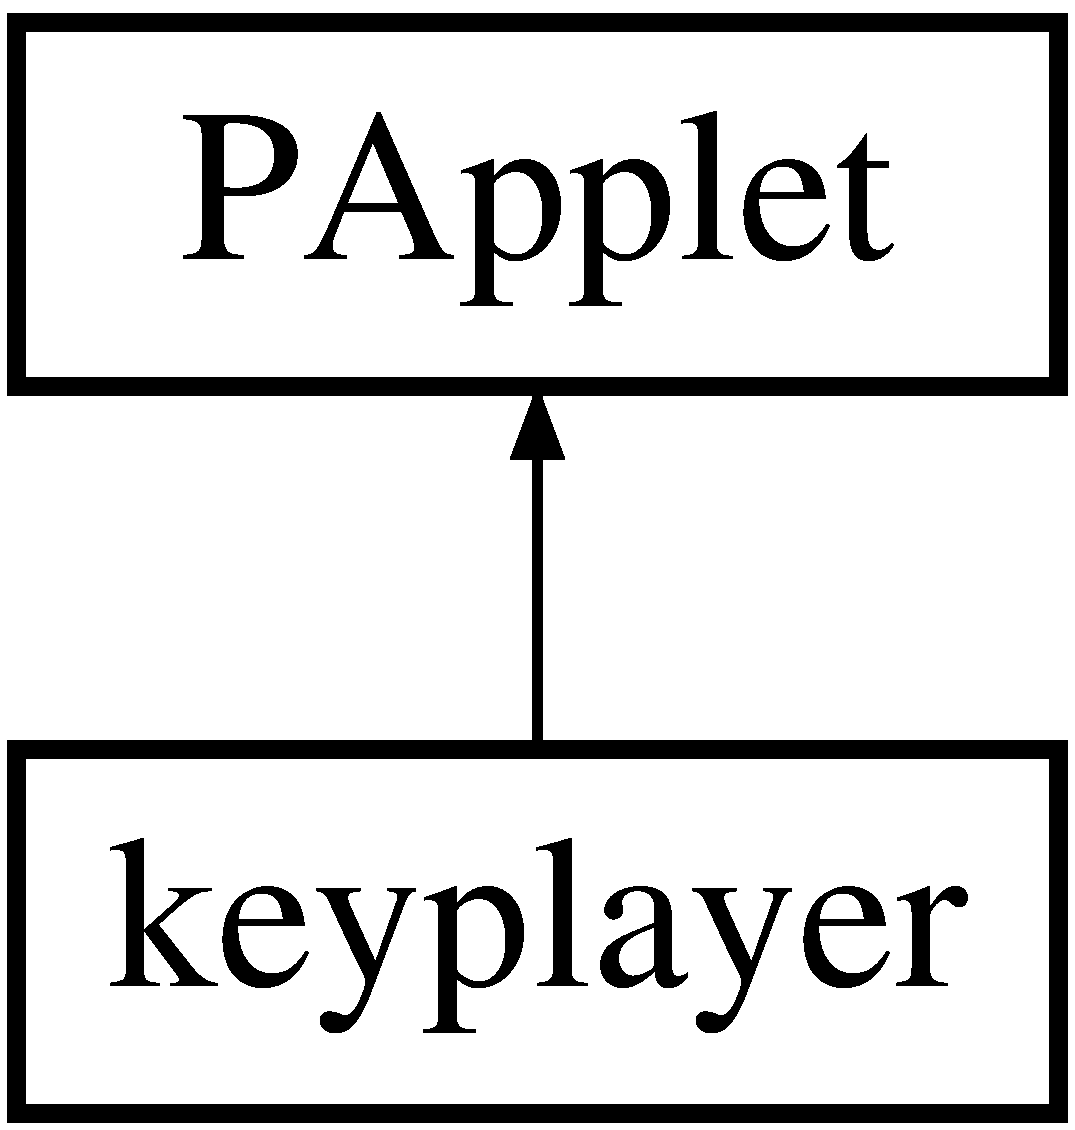
\includegraphics[height=2.000000cm]{classkeyplayer}
\end{center}
\end{figure}
\subsection*{Public Member Functions}
\begin{DoxyCompactItemize}
\item 
void \hyperlink{classkeyplayer_a0b7282386790ccfe8ca8fec9ba8b7e69}{setup} ()
\item 
void \hyperlink{classkeyplayer_a1e09a6adb89438a2ee315bef66d319e0}{draw} ()
\item 
void \hyperlink{classkeyplayer_a4845b0307a73147593abef0fecc182cd}{key\+Pressed} ()
\item 
void \hyperlink{classkeyplayer_ab22ee713ccbfff359e1c47fc190828f4}{key\+Released} ()
\item 
void \hyperlink{classkeyplayer_adae4a03190615d6f7c092f88ef61b7c5}{stop} ()
\item 
\hypertarget{classkeyplayer_adc4853d219c900ab0b1437cf6c672238}{void {\bfseries custom\+G\+U\+I} ()}\label{classkeyplayer_adc4853d219c900ab0b1437cf6c672238}

\item 
\hypertarget{classkeyplayer_a56dada7e8df126d317be2cadaf82a0b4}{void {\bfseries q\+\_\+click1} (G\+Button source, G\+Event event)}\label{classkeyplayer_a56dada7e8df126d317be2cadaf82a0b4}

\item 
\hypertarget{classkeyplayer_a3fd6957d08db95374cf73f9f28145673}{void {\bfseries w\+\_\+click1} (G\+Button source, G\+Event event)}\label{classkeyplayer_a3fd6957d08db95374cf73f9f28145673}

\item 
\hypertarget{classkeyplayer_ab8bfc95261953068b81ff477a268eba8}{void {\bfseries e\+\_\+click1} (G\+Button source, G\+Event event)}\label{classkeyplayer_ab8bfc95261953068b81ff477a268eba8}

\item 
\hypertarget{classkeyplayer_a055bd941463df838049b07734fde8742}{void {\bfseries r\+\_\+click1} (G\+Button source, G\+Event event)}\label{classkeyplayer_a055bd941463df838049b07734fde8742}

\item 
\hypertarget{classkeyplayer_a62167d49a9cc87a8166c311f6e783399}{void {\bfseries slider1\+\_\+change1} (G\+Slider source, G\+Event event)}\label{classkeyplayer_a62167d49a9cc87a8166c311f6e783399}

\item 
\hypertarget{classkeyplayer_aadd83307147b9e4920ed54ea2d11db92}{void {\bfseries t\+\_\+click1} (G\+Button source, G\+Event event)}\label{classkeyplayer_aadd83307147b9e4920ed54ea2d11db92}

\item 
\hypertarget{classkeyplayer_a97b8904a6c9400e5ea09e23df2cdb8c1}{void {\bfseries y\+\_\+click1} (G\+Button source, G\+Event event)}\label{classkeyplayer_a97b8904a6c9400e5ea09e23df2cdb8c1}

\item 
\hypertarget{classkeyplayer_a30ed151da70f312b272e8a849b02987c}{void {\bfseries u\+\_\+click1} (G\+Button source, G\+Event event)}\label{classkeyplayer_a30ed151da70f312b272e8a849b02987c}

\item 
\hypertarget{classkeyplayer_a64f074a00415060451095fbdee0b6cf9}{void {\bfseries i\+\_\+click1} (G\+Button source, G\+Event event)}\label{classkeyplayer_a64f074a00415060451095fbdee0b6cf9}

\item 
\hypertarget{classkeyplayer_a9caebe1ee81401404cffab7713c03dfd}{void {\bfseries a\+\_\+click1} (G\+Button source, G\+Event event)}\label{classkeyplayer_a9caebe1ee81401404cffab7713c03dfd}

\item 
\hypertarget{classkeyplayer_a82c4b75d1a2591b20689c8c1f276cdc1}{void {\bfseries s\+\_\+click1} (G\+Button source, G\+Event event)}\label{classkeyplayer_a82c4b75d1a2591b20689c8c1f276cdc1}

\item 
\hypertarget{classkeyplayer_a011d7ce7eb3d0f45462bcb0127c509d0}{void {\bfseries d\+\_\+click1} (G\+Button source, G\+Event event)}\label{classkeyplayer_a011d7ce7eb3d0f45462bcb0127c509d0}

\item 
\hypertarget{classkeyplayer_aca00e1a17faa1075b56c8ac3fff33abf}{void {\bfseries f\+\_\+click1} (G\+Button source, G\+Event event)}\label{classkeyplayer_aca00e1a17faa1075b56c8ac3fff33abf}

\item 
\hypertarget{classkeyplayer_ae2707922d175c92f211c1920ab7cb658}{void {\bfseries g\+\_\+click1} (G\+Button source, G\+Event event)}\label{classkeyplayer_ae2707922d175c92f211c1920ab7cb658}

\item 
\hypertarget{classkeyplayer_a9f1f12fc075f6d52afd8230f032afec2}{void {\bfseries h\+\_\+click1} (G\+Button source, G\+Event event)}\label{classkeyplayer_a9f1f12fc075f6d52afd8230f032afec2}

\item 
\hypertarget{classkeyplayer_a63525c9ed4440e27c9f7ce3ea300d2de}{void {\bfseries j\+\_\+click1} (G\+Button source, G\+Event event)}\label{classkeyplayer_a63525c9ed4440e27c9f7ce3ea300d2de}

\item 
\hypertarget{classkeyplayer_a65565c04e3f2fe3f0c3996de402db97f}{void {\bfseries k\+\_\+click1} (G\+Button source, G\+Event event)}\label{classkeyplayer_a65565c04e3f2fe3f0c3996de402db97f}

\item 
\hypertarget{classkeyplayer_a5c90178dd9aec63580115fe819090500}{void {\bfseries z\+\_\+click1} (G\+Button source, G\+Event event)}\label{classkeyplayer_a5c90178dd9aec63580115fe819090500}

\item 
\hypertarget{classkeyplayer_aaa1dd6f6e14cb159510891509b32e75c}{void {\bfseries x\+\_\+click1} (G\+Button source, G\+Event event)}\label{classkeyplayer_aaa1dd6f6e14cb159510891509b32e75c}

\item 
\hypertarget{classkeyplayer_a7a48d806f3a128e77926322bf72b958d}{void {\bfseries c\+\_\+click1} (G\+Button source, G\+Event event)}\label{classkeyplayer_a7a48d806f3a128e77926322bf72b958d}

\item 
\hypertarget{classkeyplayer_ae7a62ee5fce7b79bc9336a4ee59229d6}{void {\bfseries v\+\_\+click1} (G\+Button source, G\+Event event)}\label{classkeyplayer_ae7a62ee5fce7b79bc9336a4ee59229d6}

\item 
\hypertarget{classkeyplayer_aa1ee94f5ef57dbbf9fab15bcf1cc3322}{void {\bfseries b\+\_\+click1} (G\+Button source, G\+Event event)}\label{classkeyplayer_aa1ee94f5ef57dbbf9fab15bcf1cc3322}

\item 
\hypertarget{classkeyplayer_a5a2dfbf19de127e8309f01c6a1697f80}{void {\bfseries n\+\_\+click1} (G\+Button source, G\+Event event)}\label{classkeyplayer_a5a2dfbf19de127e8309f01c6a1697f80}

\item 
\hypertarget{classkeyplayer_a8d70fc97fb9f9ac0c83040a006cb65cf}{void {\bfseries m\+\_\+click1} (G\+Button source, G\+Event event)}\label{classkeyplayer_a8d70fc97fb9f9ac0c83040a006cb65cf}

\item 
\hypertarget{classkeyplayer_a55d77ebad7ffd34187619fb6cd732f4c}{void {\bfseries drop\+List1\+\_\+click1} (G\+Drop\+List source, G\+Event event)}\label{classkeyplayer_a55d77ebad7ffd34187619fb6cd732f4c}

\item 
\hypertarget{classkeyplayer_a4ad43a875652d9e80bd48e54c0a9b8fe}{void {\bfseries comma\+\_\+click1} (G\+Button source, G\+Event event)}\label{classkeyplayer_a4ad43a875652d9e80bd48e54c0a9b8fe}

\item 
\hypertarget{classkeyplayer_aedef180177a9e5b77173626a0f5bda08}{void {\bfseries create\+G\+U\+I} ()}\label{classkeyplayer_aedef180177a9e5b77173626a0f5bda08}

\end{DoxyCompactItemize}
\subsection*{Static Public Member Functions}
\begin{DoxyCompactItemize}
\item 
\hypertarget{classkeyplayer_ab9305405f2bdc53c4b9ded37677ec901}{static void {\bfseries main} (String\mbox{[}$\,$\mbox{]} passed\+Args)}\label{classkeyplayer_ab9305405f2bdc53c4b9ded37677ec901}

\end{DoxyCompactItemize}


\subsection{Member Function Documentation}
\hypertarget{classkeyplayer_a1e09a6adb89438a2ee315bef66d319e0}{\index{keyplayer@{keyplayer}!draw@{draw}}
\index{draw@{draw}!keyplayer@{keyplayer}}
\subsubsection[{draw}]{\setlength{\rightskip}{0pt plus 5cm}void keyplayer.\+draw (
\begin{DoxyParamCaption}
{}
\end{DoxyParamCaption}
)}}\label{classkeyplayer_a1e09a6adb89438a2ee315bef66d319e0}
\hyperlink{classkeyplayer_a1e09a6adb89438a2ee315bef66d319e0}{draw()} adds visual elements to the G\+U\+I.\hypertarget{classkeyplayer_a4845b0307a73147593abef0fecc182cd}{\index{keyplayer@{keyplayer}!key\+Pressed@{key\+Pressed}}
\index{key\+Pressed@{key\+Pressed}!keyplayer@{keyplayer}}
\subsubsection[{key\+Pressed}]{\setlength{\rightskip}{0pt plus 5cm}void keyplayer.\+key\+Pressed (
\begin{DoxyParamCaption}
{}
\end{DoxyParamCaption}
)}}\label{classkeyplayer_a4845b0307a73147593abef0fecc182cd}
\hyperlink{classkeyplayer_a4845b0307a73147593abef0fecc182cd}{key\+Pressed()} is the main function of the program. It parses keyboard input and displays the visual effects for each key and plays the correct note.

press 1 to load heyheyhey.\+wav

press 2 to load Scary Monsters and Nice Sprites.\+mp3

press 3 to load Chip on Your Shoulder.\+mp3

press 4 to load Closer.\+mp3

then press spacebar to play the song! \hypertarget{classkeyplayer_ab22ee713ccbfff359e1c47fc190828f4}{\index{keyplayer@{keyplayer}!key\+Released@{key\+Released}}
\index{key\+Released@{key\+Released}!keyplayer@{keyplayer}}
\subsubsection[{key\+Released}]{\setlength{\rightskip}{0pt plus 5cm}void keyplayer.\+key\+Released (
\begin{DoxyParamCaption}
{}
\end{DoxyParamCaption}
)}}\label{classkeyplayer_ab22ee713ccbfff359e1c47fc190828f4}
\hyperlink{classkeyplayer_ab22ee713ccbfff359e1c47fc190828f4}{key\+Released()} updates the visualizer on key release.\hypertarget{classkeyplayer_a0b7282386790ccfe8ca8fec9ba8b7e69}{\index{keyplayer@{keyplayer}!setup@{setup}}
\index{setup@{setup}!keyplayer@{keyplayer}}
\subsubsection[{setup}]{\setlength{\rightskip}{0pt plus 5cm}void keyplayer.\+setup (
\begin{DoxyParamCaption}
{}
\end{DoxyParamCaption}
)}}\label{classkeyplayer_a0b7282386790ccfe8ca8fec9ba8b7e69}
\hyperlink{classkeyplayer_a0b7282386790ccfe8ca8fec9ba8b7e69}{setup()} builds the initial frame for the program by opening in fullscreen mode and initiating the G\+U\+I.\hypertarget{classkeyplayer_adae4a03190615d6f7c092f88ef61b7c5}{\index{keyplayer@{keyplayer}!stop@{stop}}
\index{stop@{stop}!keyplayer@{keyplayer}}
\subsubsection[{stop}]{\setlength{\rightskip}{0pt plus 5cm}void keyplayer.\+stop (
\begin{DoxyParamCaption}
{}
\end{DoxyParamCaption}
)}}\label{classkeyplayer_adae4a03190615d6f7c092f88ef61b7c5}
\hyperlink{classkeyplayer_adae4a03190615d6f7c092f88ef61b7c5}{stop()} stops key sounds on key release.

The documentation for this class was generated from the following file\+:\begin{DoxyCompactItemize}
\item 
keyplayer/application.\+linux64/source/keyplayer.\+java\end{DoxyCompactItemize}

%--- End generated contents ---

% Index
\newpage
\phantomsection
\addcontentsline{toc}{chapter}{Index}
\printindex

\end{document}
